\section{Method}
\label{sec:method}

In this section we will look on how to implement the circuit using transistors and logic gates. 

\subsection{Circuit design}
\label{subsec:circuitDesign}

When designing the different componenents for the circuit, we will logic gates to 

% The Multiply accumulate circuit can be divided into different subsystems. In this section we are going to explain the functions of each subsystem and create a circuit design to implement in later sections. In figure \ref{fig:blokk} the different subsystems are shown and how they connect. 

% \begin{figure}[H]
%     \centering
%     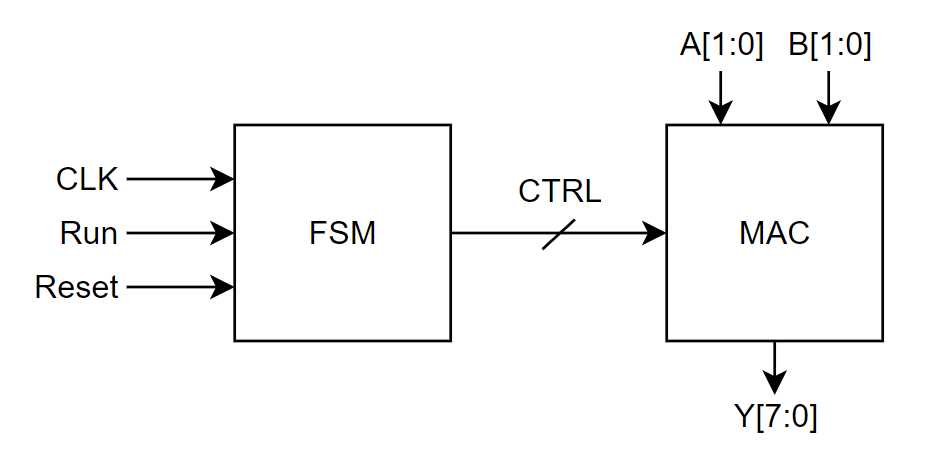
\includegraphics[width=0.7\textwidth]{Figures/Blokk.png}
%     \caption{An overview of the complete system.}
%     \label{fig:blokk}
% \end{figure}

\subsubsection{MAC Unit}


% The equation that the MAC unit are going to use is

% \begin{equation}
%     C \leftarrow C + (A \cdot B)
% \end{equation}

% The MAC unit will receive two 2-bit inputs, A and B, which will be multiplied and added to C. This should happen every rising edge of the clock. The MAC unit consist of a multiplier, an adder and an accumulator. The layout of the MAC is shown in figure \ref{fig:mac-blokk}. 
% \begin{figure}[htpb]
%     \centering
%     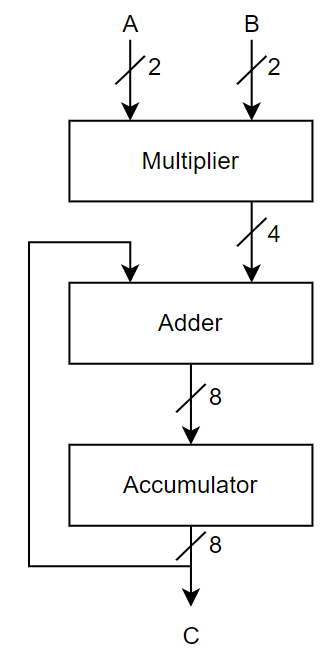
\includegraphics[width=0.3\textwidth]{Figures/mac-blokk.png}
%     \caption{Layout of MAC unit}
%     \label{fig:mac-blokk}
% \end{figure}

\paragraph{Multiplier}
% The multiplier takes in A and B, two 2 bits inputs, and multiply them. The value of A times B can't be higher than 9, which means that the output of the multiplier has to be at least 4 bits. 

A 2-bit multiplier could be designed like shown in figure \ref{fig:multiplier}.

\begin{figure}[H]
    \centering
    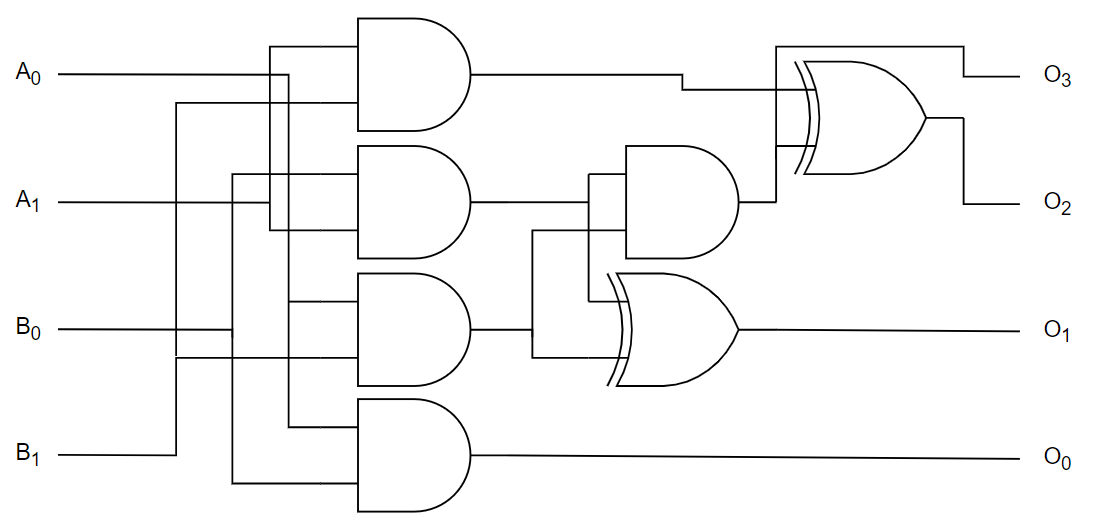
\includegraphics[width=0.8\textwidth]{Figures/multiplier.png}
    \caption{Possible design of multiplier}
    \label{fig:multiplier}
\end{figure}

\paragraph{Adder}
% As shown in figure \ref{fig:mac-blokk}, the adder has to take the sum of a 4-bit number and a 8-bit number. The design of an 8-bit adder is shown in figure \ref{fig:adder-blokk}. The figure shows two 8-bit numbers A and B, and their sum S with a carry $C_O$. 


The circuit for the half and full adder is shown in figure \ref{fig:halfadder} and \ref{fig:fulladder}.

\begin{figure}[H]
\begin{minipage}{0.4\textwidth}
    \centering
    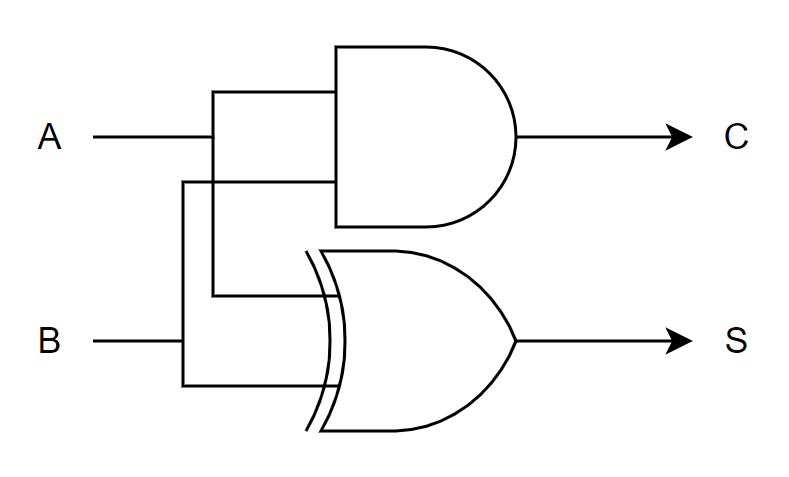
\includegraphics[width=\linewidth]{Figures/halfadder.png}
    \caption{Half adder}
    \label{fig:halfadder}
\end{minipage}
\begin{minipage}{0.6\textwidth}
    \centering
    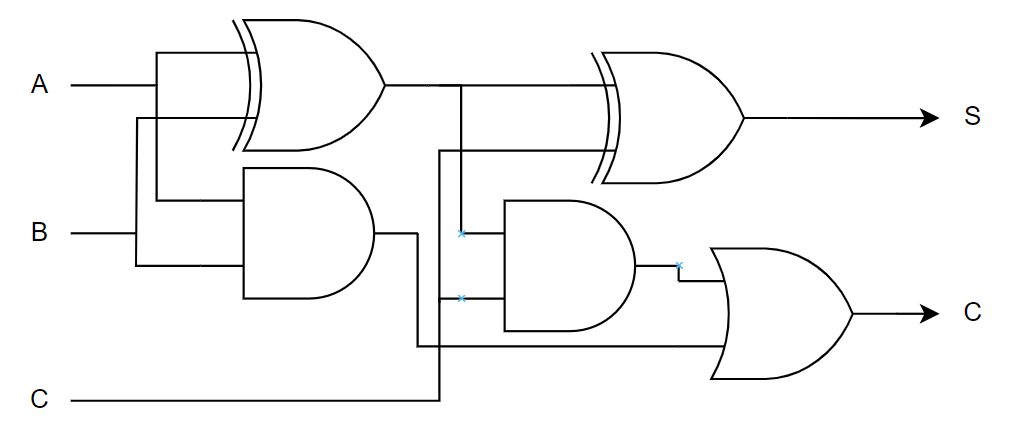
\includegraphics[width=\linewidth]{Figures/fulladder.png}
    \caption{Full adder}
    \label{fig:fulladder}
\end{minipage}
\end{figure}



\paragraph{Accumulator}
The accumulator is an 8-bit register with some control signals, that is received from the Final State Machine (FSM). 

\begin{figure}[H]
    \centering
    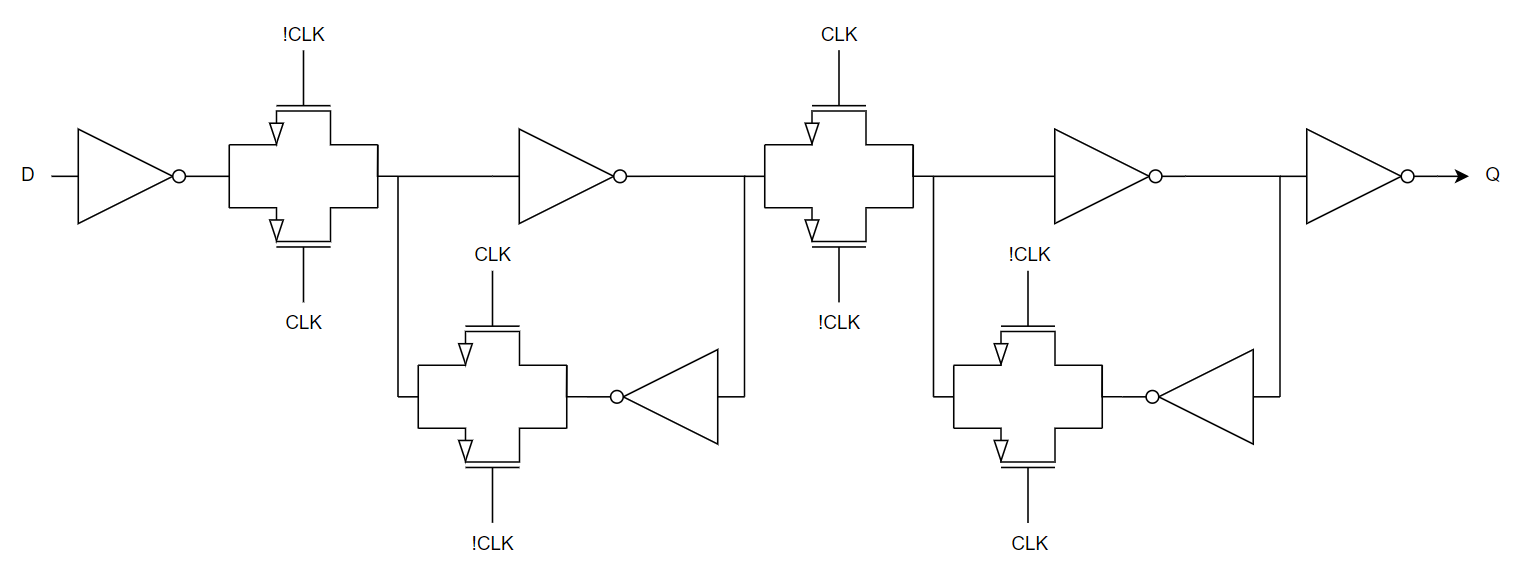
\includegraphics[width=\textwidth]{Figures/D_Flip_Flop.png}
    \caption{D-flip flop}
    \label{fig:dflipflop}
\end{figure}

\begin{figure}[H]
    \centering
    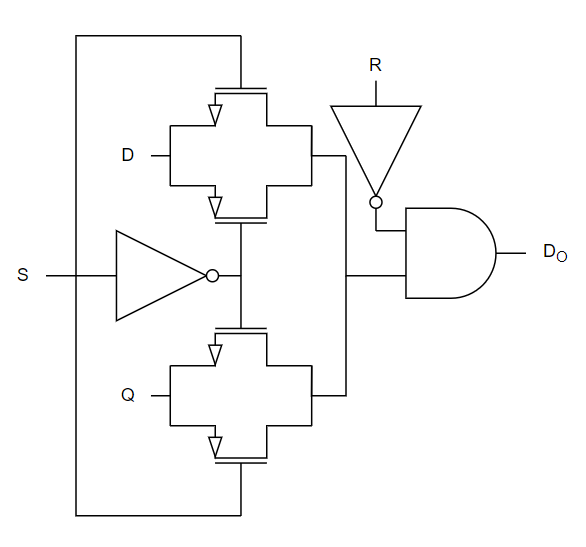
\includegraphics[width=0.7\textwidth]{Figures/setReset.png}
    \caption{Circuit for controlling register}
    \label{fig:setreset}
\end{figure}



\subsection{AimSpice}
In the AimSpice related part of the assignment, a 1 bit register will be implemented using the designs shown in section \ref{subsec:circuitDesign}. 

To implement the register in AimSpice, different logic gates are made using transistors. The different logic gates used in the 1-bit register are NOT, AND and transmission gates. This is shown in figure \ref{fig:dflipflop} and \ref{fig:setreset}.

\begin{figure}[H]
\begin{minipage}{0.5\textwidth}
    \centering
    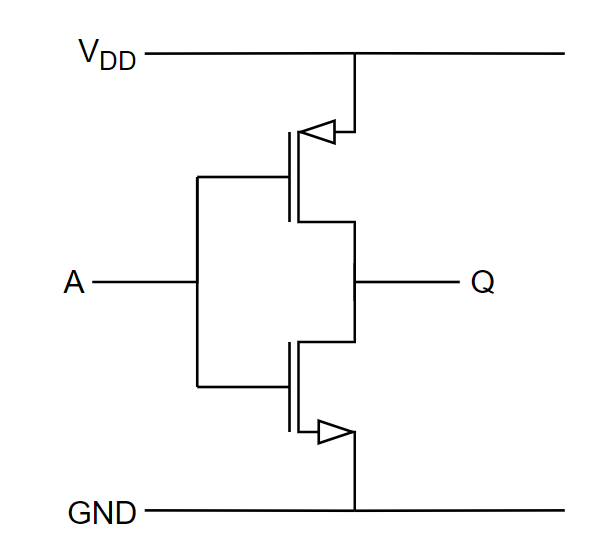
\includegraphics[width=\linewidth]{Figures/Not gate.png}
    \caption{NOT gate using MOSFET}
    \label{fig:NOT}
\end{minipage}
\begin{minipage}{0.5\textwidth}
    \centering
    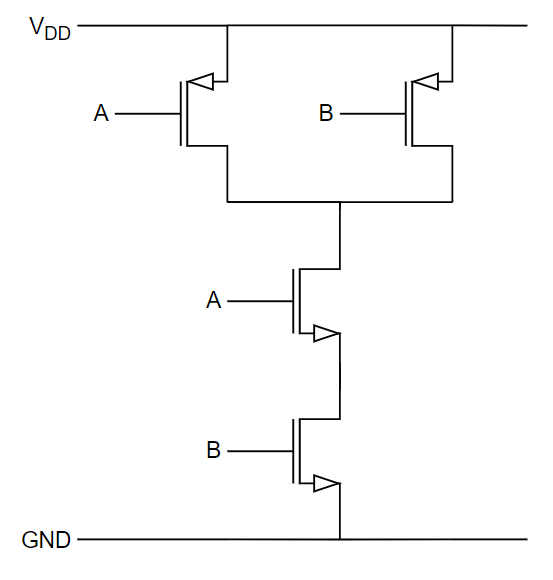
\includegraphics[width=\linewidth]{Figures/Nand Gate.png}
    \caption{NAND gate using MOSFET}
    \label{fig:NAND}
\end{minipage}
\end{figure}

The AND gate is made by connecting a NAND and NOT in series, as shown in figure \ref{fig:AND}.
\begin{figure}[H]
    \centering
    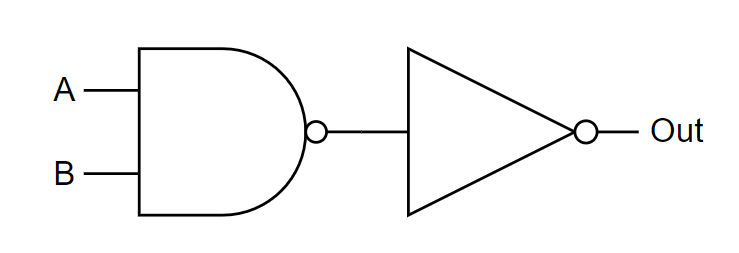
\includegraphics[width=0.4\linewidth]{Figures/And gate.png}
    \caption{AND gate}
    \label{fig:AND}
\end{figure}



\subsection{Verilog}


\subsubsection{Finite State Machine}
\label{subsec:fsm_}

Three input signals are given by the project description~\cite{project_description}, Reset, CLK and Run. The CLK-signal will only be used to time the sequential logic in the FSM and passed on to the MAC unit without further modification.

The resulting FSM will therefore recieve a 2-bit input, Reset($I_1$) and Run($I_0$). For the control signals between the FSM and the MAC unit, we have chosen a 2-bit signal consisting of Control-Reset($O_1$) and Control-Run($O_0$). 

A Moore FSM is chosen as the preffered FSM model. In general, a Moore FSM is power-efficient in terms of static power consumption compared to a Mealy FSM. This is because Moore machines typically have outputs that are associated only with states, and they remain stable for the entire duration of a state. As a result, there are fewer transitions and less activity in the output logic, leading to lower static power consumption.

Following the detailed description of the FSM's functionality in section 2.2.1 in the project description~\cite{project_description}, and the design procediure given in~\ref{subsec:fsm_theory}, the resulting FSM requires seven different states 0-6. Thus, the FSM needs a 3-bit register. A general topology is shown in figure~\ref{fig:fsm_overordnet}

\begin{figure}[H]
    \centering
    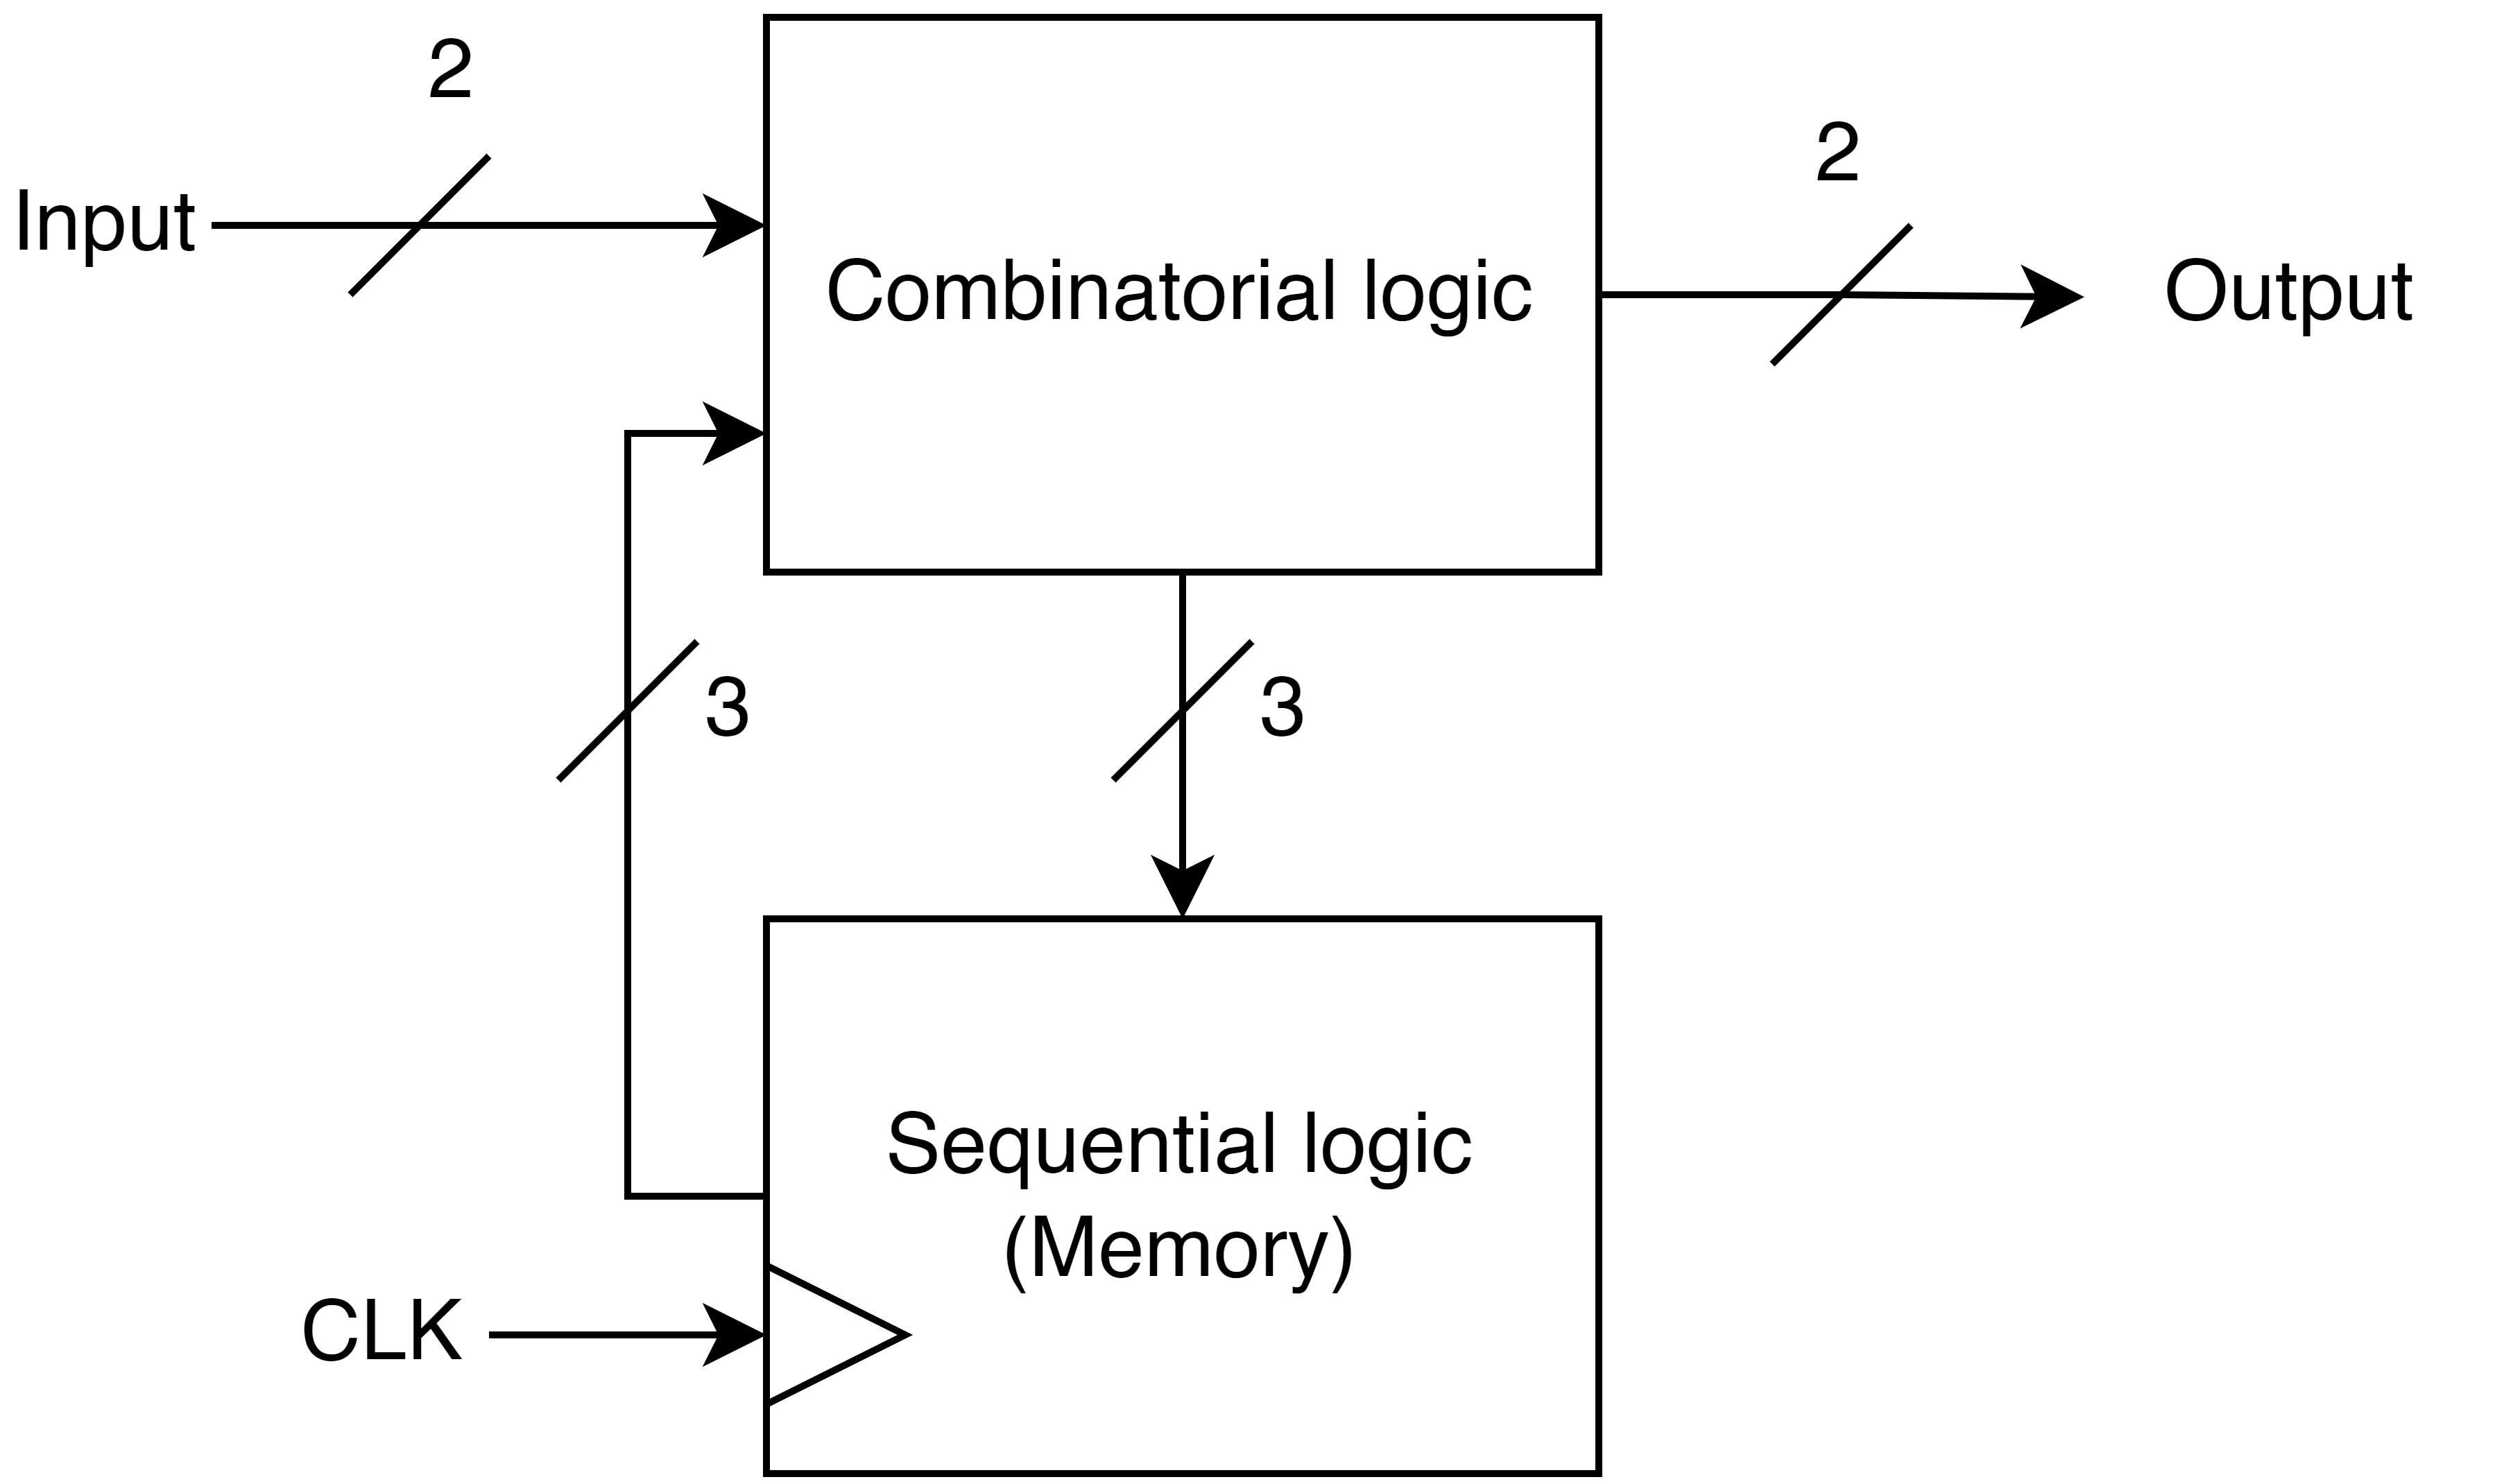
\includegraphics[width=0.6\textwidth]{Figures/FSM_overordnet.drawio.png}
    \caption{FSM general topology diagram}
    \label{fig:fsm_overordnet}
\end{figure}

The current state is from here described by the three signals $C_2$, $C_1$ and $C_0$. The next state is describrd by the three signals $N_2$, $N_1$ and $N_0$.

Figure~\ref{fig:fsm_diagram} and table~\ref{tab:truthtable} show a detailed overview of the wanted functionality of the FSM, describing the relation between inputs, outputs, current state and next state. Transitions for each current state and input is described by arrows, and output is described within each state ($C_2 C_1 C_0$/$O_1 O_0$)

\begin{figure}[H]
    \centering
    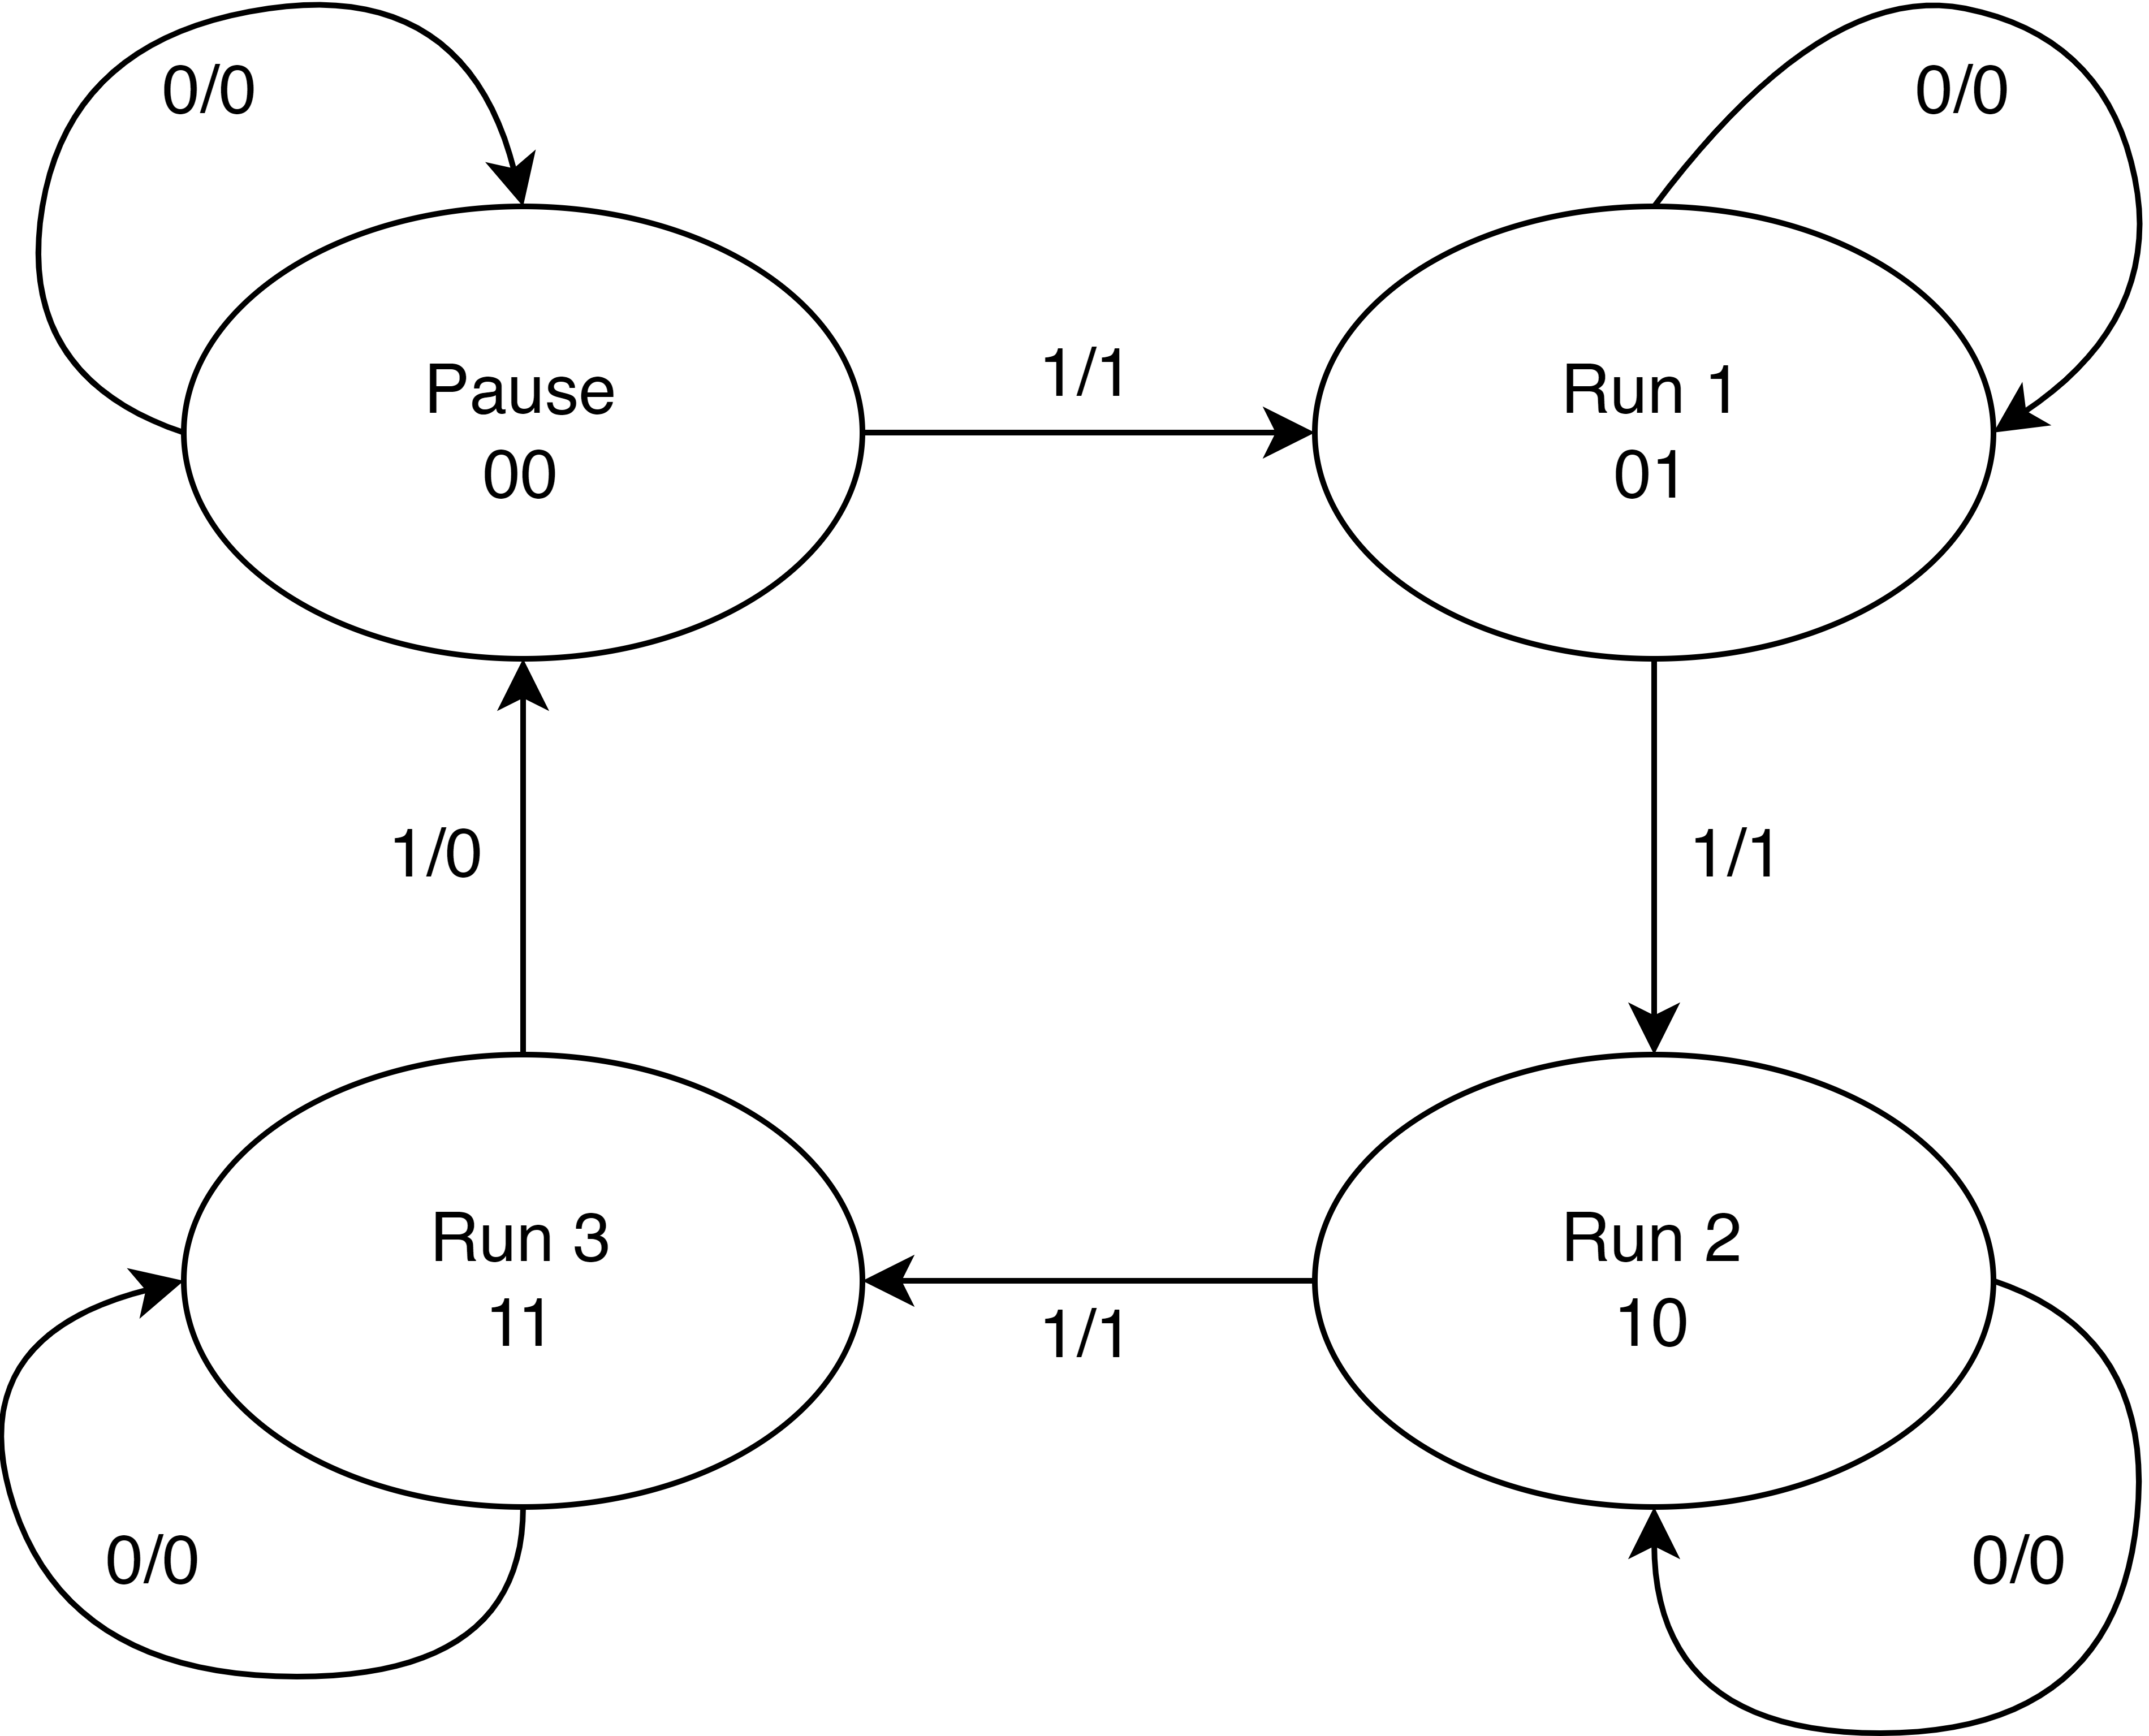
\includegraphics[width=0.8\textwidth]{Figures/FSM-diagram.png}
    \caption{FSM Diagram}
    \label{fig:fsm_diagram}
\end{figure}

\begin{table}[H]
\caption{Truth table for the FSM}
\label{tab:truthtable}
\centering
\begin{tabular}{|l|l|l|l|l|l|l|l|l|l|}
\hline
\rowcolor[HTML]{C0C0C0} 
$C_2$ & $C_1$ & $C_0$ & $I_1$ & $I_0$ & $N_2$ & $N_1$ & $N_0$ & $O_1$ & $O_0$ \\ \hline
0  & 0  & 0  & 0   & 0   & 0  & 0  & 0  & 0   & 0   \\ \hline
0  & 0  & 0  & 0   & 1   & 0  & 0  & 1  & 0   & 0   \\ \hline
0  & 0  & 0  & 1   & 0   & 1  & 1  & 0  & 0   & 0   \\ \hline
0  & 0  & 0  & 1   & 1   & 1  & 1  & 0  & 0   & 0   \\ \hline
0  & 0  & 1  & 0   & 0   & 1  & 0  & 0  & 0   & 1   \\ \hline
0  & 0  & 1  & 0   & 1   & 0  & 1  & 0  & 0   & 1   \\ \hline
0  & 0  & 1  & 1   & 0   & 1  & 1  & 0  & 0   & 1   \\ \hline
0  & 0  & 1  & 1   & 1   & 1  & 1  & 0  & 0   & 1   \\ \hline
0  & 1  & 0  & 0   & 0   & 1  & 0  & 1  & 0   & 1   \\ \hline
0  & 1  & 0  & 0   & 1   & 0  & 1  & 1  & 0   & 1   \\ \hline
0  & 1  & 0  & 1   & 0   & 1  & 1  & 0  & 0   & 1   \\ \hline
0  & 1  & 0  & 1   & 1   & 1  & 1  & 0  & 0   & 1   \\ \hline
0  & 1  & 1  & 0   & 0   & 0  & 0  & 0  & 0   & 1   \\ \hline
0  & 1  & 1  & 0   & 1   & 0  & 0  & 0  & 0   & 1   \\ \hline
0  & 1  & 1  & 1   & 0   & 1  & 1  & 0  & 0   & 1   \\ \hline
0  & 1  & 1  & 1   & 1   & 1  & 1  & 0  & 0   & 1   \\ \hline
1  & 0  & 0  & 0   & 0   & 1  & 0  & 0  & 0   & 0   \\ \hline
1  & 0  & 0  & 0   & 1   & 0  & 1  & 0  & 0   & 0   \\ \hline
1  & 0  & 0  & 1   & 0   & 1  & 1  & 0  & 0   & 0   \\ \hline
1  & 0  & 0  & 1   & 1   & 1  & 1  & 0  & 0   & 0   \\ \hline
1  & 0  & 1  & 0   & 0   & 1  & 0  & 1  & 0   & 0   \\ \hline
1  & 0  & 1  & 0   & 1   & 0  & 1  & 1  & 0   & 0   \\ \hline
1  & 0  & 1  & 1   & 0   & 1  & 1  & 0  & 0   & 0   \\ \hline
1  & 0  & 1  & 1   & 1   & 1  & 1  & 0  & 0   & 0   \\ \hline
1  & 1  & 0  & 0   & 0   & 0  & 0  & 0  & 1   & 0   \\ \hline
1  & 1  & 0  & 0   & 1   & 0  & 0  & 1  & 1   & 0   \\ \hline
1  & 1  & 0  & 1   & 0   & 1  & 1  & 0  & 1   & 0   \\ \hline
1  & 1  & 0  & 1   & 1   & 1  & 1  & 0  & 1   & 0   \\ \hline
\end{tabular}
\end{table}



In this section you should explain what you have done, and how you have done it. The explanations should have enough detail to make a reproduction possible (i.e. it should be possible to do exactly what you have done, and receive the same results, only by doing what you write in this section).


It might be relevant to refer back to a part of theory, as explained in \autoref{subsec:theory_aSubsection}, to explain the design choices you made.

\subsection{Must include}
The method section MUST INCLUDE:
\begin{itemize}
    \item One or more illustrations showing your circuit. As a minimum you must include one figure of the circuit at the logic gate level, and one of what you implemented at transistor level in AIMSpice.
    \item Figure showing the state diagram for your final state machine (FSM).
    \item Explanations of design choices you made when creating the circuit.
    \item Explanations of the simulations you did (not the results, just how they were done).
\end{itemize}